%%%%%%%%%%%%%%%%%%%%%%%%%%%%%%%%%%%%%%%%%%%%%%%%%%%%%%%%%%%%%%%%%%%%%%%%%%%
%  DSM SF-PBL FRONTIERS IN EDUCATION — FINAL MANUSCRIPT
%  Template: FrontiersinHarvard.cls (v3.4, official Frontiers template)
%  Journal:  Frontiers in Education — STEM Education Section
%  Type:     Original Research Article
%  Author:   Sunny Nanade | NMIMS MPSTME, Mumbai
%  Date:     2026-07-25 | All statistics verified from raw CSV + Excel
%%%%%%%%%%%%%%%%%%%%%%%%%%%%%%%%%%%%%%%%%%%%%%%%%%%%%%%%%%%%%%%%%%%%%%%%%%%

\documentclass[utf8]{FrontiersinHarvard}

\usepackage{url,hyperref,lineno,microtype,subcaption}
\usepackage[onehalfspacing]{setspace}
\usepackage{booktabs}
\usepackage{array}
\usepackage{multirow}
\usepackage{amsmath}
\usepackage{amssymb}
\usepackage{graphicx}
\usepackage{paralist}

\linenumbers

%%% ─── AUTHOR / AFFILIATION BLOCK ────────────────────────────────────────
\def\keyFont{\fontsize{8}{11}\helveticabold}

\def\firstAuthorLast{Nanade {et~al.}}

\def\Authors{Sunny Nanade\,$^{1*}$, Debasis Dash\,$^{1}$, Sudipto Sarkar\,$^{1}$ and Koteswararao Anne\,$^{1}$}

\def\Address{%
  $^{1}$Mukesh Patel School of Technology Management \& Engineering,
  SVKM's NMIMS, Mumbai, India}

\def\corrAuthor{Sunny Nanade}
\def\corrEmail{sunny.nanade@nmims.edu}

%%% ─── DOCUMENT START ────────────────────────────────────────────────────
\begin{document}
\onecolumn
\firstpage{1}

\title[SF-PBL for Engineering Dynamics]{%
  A Computationally-Integrated Simulation-Focused Problem-Based Learning
  Framework for Engineering Dynamics: Design, Implementation, and
  Mixed-Methods Evaluation in an OBE-Aligned Undergraduate Course}

\author[\firstAuthorLast]{\Authors}
\address{}
\correspondance{}
\extraAuth{}

\maketitle

%%% ─── ABSTRACT ──────────────────────────────────────────────────────────
\begin{abstract}

\section{}

Engineering dynamics courses demand simultaneous development of mathematical
modelling, computational implementation, and communication competencies, yet
conventional instruction rarely provides authentic contexts for their
integration. This study presents the design, implementation, and
mixed-methods evaluation of a Simulation-Focused Problem-Based Learning
(SF-PBL) framework embedded within a 15-week undergraduate Dynamic System
Modeling (DSM) course ($N$\,=\,53, B.Tech Mechatronics Engineering, Semester
IV, January--April 2026) at an NBA-accredited institution in India. The
framework operationalises a four-phase computational pipeline---System
Identification, Mathematical Modelling, Computational Simulation,
Validation \& Communication---scaffolded through an Explain-Try-Challenge
(E-T-C) model and assessed via a six-judge external expert panel. A
pre--post mixed-methods design measured self-efficacy (10-item Likert
scale), conceptual knowledge (5-item MCQ), PBL satisfaction, AI tool
usage, and qualitative breakthrough reflections. Self-efficacy improved
significantly (pre: $M$\,=\,2.92, $SD$\,=\,0.21; post: $M$\,=\,3.80,
$SD$\,=\,0.40; $t$(52)\,=\,13.91, $p$\,$<$\,.001, Cohen's $d$\,=\,2.72,
pooled SD). Knowledge gains were large ($t$(52)\,=\,11.32, $p$\,$<$\,.001,
$d$\,=\,1.20; Hake's $g$\,=\,0.50, medium interactive-engagement band).
All ten self-efficacy items improved significantly ($p$\,$<$\,.001). PBL
satisfaction was high ($M$\,=\,3.74, $SD$\,=\,0.30). Eighty-five percent
of students used AI tools, primarily for computational coding, while
mathematical derivation remained predominantly human-led. Qualitative
themes identified simulation validation, PID tuning, and linking derivation
to computation as universal breakthrough moments. Exhibition rubric scores
from 17 student projects evaluated by the six-judge panel ($M$\,=\,82.62/100,
$SD$\,=\,9.98) confirmed strong authentic performance. The SF-PBL framework
provides a replicable, evidence-based model for computationally-integrated
dynamics pedagogy in OBE-aligned STEM programmes.

\tiny
\keyFont{\section{Keywords:}
  problem-based learning; engineering dynamics; computational simulation;
  self-efficacy; OBE; authentic assessment; AI-assisted learning;
  STEM education}

\end{abstract}

%%% ═══════════════════════════════════════════════════════════════════════
\section{Introduction}
%%% ═══════════════════════════════════════════════════════════════════════

\subsection{The Pedagogical Challenge in Engineering Dynamics}

Engineering dynamics---encompassing kinematics, constitutive laws, Lagrangian
mechanics, and vibration analysis---occupies a foundational position in
mechanical and mechatronics engineering curricula worldwide. Despite its
centrality, the course presents persistent and well-documented pedagogical
challenges: the mathematical formalism is demanding, physical intuition is
difficult to develop, and the connection between abstract theory and real
engineering systems is rarely made explicit within traditional lecture-driven
instruction \citep{streveler2008learning}. Withdrawal, failure, and
incomplete (DFW) rates in core dynamics and mechanics courses at
undergraduate level remain a persistent concern, with some institutions
reporting DFW rates exceeding 20--30\% in introductory engineering
mechanics sequences \citep{crisp2009increasing}. Students frequently navigate
these courses through surface-level pattern-matching without building the
conceptual depth required for engineering practice.

Compounding this challenge is the increasing centrality of computational
tools in modern engineering practice. Graduates are expected not only to
derive equations of motion analytically but to implement them numerically,
simulate dynamic system behaviour across time domains, and interpret
computational outputs as engineering evidence---a set of competencies that
conventional closed-book assessments rarely evaluate authentically
\citep{justo2021enhancing}. The emergence of AI-assisted coding tools
(ChatGPT, GitHub Copilot, Claude Sonnet) has further transformed the
competency landscape: students can now generate working simulation code in
seconds, fundamentally shifting the pedagogical question from
\textit{``can you write the code?''} to \textit{``do you understand what
the code is computing and why?''} \citep{tlili2023chatgpt}.

\subsection{Problem-Based Learning in Engineering: Promise and Gap}

Problem-Based Learning (PBL), as defined by \citet{hmelo2004problem}, places
authentic, ill-structured problems at the centre of learning, requiring
students to self-direct their inquiry, build domain knowledge collaboratively,
and communicate solutions to real audiences. In engineering education, PBL
has consistently demonstrated improvements in conceptual understanding,
motivation, and collaborative problem-solving competencies compared to
conventional instruction \citep{prince2006inductive, dym2005engineering,
dochy2003effects}. \citet{freeman2014active} meta-analysed 225 studies and
found that active learning produced a mean Cohen's $d$\,=\,0.47 improvement
in examination performance relative to traditional lecturing, with
engineering courses showing the strongest effect.

However, three specific implementation gaps persist in the published
literature on PBL in engineering dynamics and related computationally
intensive courses. First, most PBL implementations position a physical
prototype or design report as the primary learning artefact---rarely is
mathematical derivation from first principles and its computational
simulation verification foregrounded as the core intellectual product.
Second, authentic assessment in PBL contexts typically relies on faculty
panels or peer evaluation, with multi-domain external expert panels
covering industry, intellectual property, and communication remaining
uncommon. Third, while many institutions operate under Outcome-Based
Education (OBE) frameworks mandated by accreditation bodies such as
NBA (India) and ABET (USA), explicit and auditable traceability from
Course Outcomes through Bloom's taxonomy levels to rubric dimensions
is rarely demonstrated empirically.

\subsection{Research Questions}

This study addresses these gaps through the design, implementation, and
empirical evaluation of a Simulation-Focused Problem-Based Learning
(SF-PBL) framework. Three research questions guided the study:

\begin{itemize}\setlength{\itemsep}{0pt}\setlength{\parskip}{0pt}
  \item \textbf{RQ1:} Does the SF-PBL framework produce statistically
    significant and practically meaningful gains in students' self-efficacy
    for dynamic system modelling competencies?
  \item \textbf{RQ2:} Does the SF-PBL framework produce statistically
    significant gains in conceptual knowledge of dynamics principles?
  \item \textbf{RQ3:} How do students integrate AI tools within the
    SF-PBL structure, and what qualitative experiences characterise their
    learning breakthroughs?
\end{itemize}

\subsection{Contributions}

This paper makes four original contributions to the engineering education
literature: (1)~a documented, replicable four-phase SF-PBL computational
algorithm with full CO$\rightarrow$Bloom's$\rightarrow$NBA Programme
Outcome traceability; (2)~an authentic assessment model using a
six-domain external expert panel; (3)~empirical evidence of large-to-very-large
learning gains ($d$\,$>$\,1.0) from a rigorous pre--post mixed-methods study
($N$\,=\,53); and (4)~a characterisation of emergent human--AI
complementarity within a structured PBL framework.

%%% ═══════════════════════════════════════════════════════════════════════
\section{Theoretical Framework}
%%% ═══════════════════════════════════════════════════════════════════════

\subsection{Simulation-Focused Problem-Based Learning (SF-PBL)}

SF-PBL is defined in this study as a variant of PBL in which
\textbf{mathematical derivation from first principles and its subsequent
computational simulation constitute the primary learning artefact}. This
distinguishes SF-PBL from conventional project-based learning (where the
product is a physical prototype or design report) and from standalone
computational modelling courses (where system identification and mathematical
modelling steps are typically pre-specified by the instructor rather than
student-led).

The SF-PBL framework rests on three interlocking theoretical pillars.
\textit{First}, \textbf{Hmelo-Silver's PBL cycle} \citeyearpar{hmelo2004problem}:
students encounter an authentic, ill-structured engineering system
(student-selected), engage in self-directed inquiry to identify governing
physics, construct knowledge through mathematical and computational means,
and reflect collaboratively on computational outcomes and their physical
interpretations. \textit{Second}, \textbf{Bandura's self-efficacy theory}
\citeyearpar{bandura1997self}: mastery experiences---successfully deriving
equations of motion and observing their agreement with simulation
output---constitute the most potent mechanism for building domain-specific
self-efficacy. The four sequential SF-PBL phases provide escalating mastery
experiences mapped directly to Course Outcomes, ensuring that self-efficacy
is built incrementally and is domain-specific rather than generalised.
\textit{Third}, \textbf{Hake's interactive-engagement framework}
\citeyearpar{hake1998interactive}: courses that require active student
engagement with phenomena---rather than passive reception of
lecturer-transmitted information---systematically outperform traditional
instruction on normalised conceptual gain. SF-PBL's four-phase structure,
requiring active derivation, numerical implementation, and public defence
of results, is designed to achieve medium-to-high interactive-engagement
gain.

Underpinning these three pillars is a constructivist epistemology rooted in
Vygotsky's concept of the Zone of Proximal Development (ZPD)
\citep{vygotsky1978mind}: the E-T-C instructional model (§\ref{sec:etc})
provides dynamic scaffolding within students' ZPD, systematically reducing
support as competence develops across the 15-week course. Kolb's
\citeyearpar{kolb1984experiential} experiential learning cycle---Concrete
Experience $\rightarrow$ Reflective Observation $\rightarrow$ Abstract
Conceptualisation $\rightarrow$ Active Experimentation---maps directly onto
the four SF-PBL phases, providing a further theoretical grounding for the
sequential pipeline design.

\subsection{OBE Framework and NBA Alignment}

The DSM course was designed using OBE principles \citep{spady1994outcome}
with explicit backward design from NBA Programme Outcomes (POs) to Course
Outcomes (COs) to assessment rubric dimensions. Five COs were defined
(Table~\ref{tab:cos}), each assigned a Bloom's taxonomy level and mapped to
the relevant NBA PO.

\begin{table}[h]
\caption{Course Outcomes, Bloom's Taxonomy Levels, and NBA Programme Outcome Mapping}
\label{tab:cos}
\begin{tabular}{clcc}
\toprule
\textbf{CO} & \textbf{Statement} & \textbf{Bloom's} & \textbf{NBA PO} \\
\midrule
CO1 & Apply kinematic analysis to multi-body systems            & Apply (L3)    & PO1, PO2 \\
CO2 & Construct FBDs for complex dynamic mechanisms             & Analyse (L4)  & PO1, PO2 \\
CO3 & Derive equations of motion using Newton's laws            & Analyse (L4)  & PO1, PO2 \\
CO4 & Apply Lagrangian mechanics to holonomic systems           & Evaluate (L5) & PO1, PO2 \\
CO5 & Implement ODE solvers in Python and validate simulations  & Create (L6)   & PO2, PO5 \\
\bottomrule
\multicolumn{4}{l}{\small PO1 = Engineering Knowledge; PO2 = Problem Analysis; PO5 = Modern Tool Usage.}
\end{tabular}
\end{table}

\subsection{The Explain-Try-Challenge (E-T-C) Instructional Model}
\label{sec:etc}

Each 90-minute lecture session followed a three-phase active-learning
structure \citep{prince2006inductive}: \textbf{Explain} (30~min)---conceptual
introduction with worked examples on the whiteboard; \textbf{Try}
(40~min)---guided structured practice using Jupyter notebooks with worked-example
scaffolds; \textbf{Challenge} (20~min)---an open-ended, unseen problem
connecting the lecture content to the student's own SF-PBL project system,
requiring them to apply the newly introduced concept to their self-selected
engineering system. The Challenge phase operationalised Vygotsky's ZPD:
it consistently targeted skills just beyond students' independent capability,
making the weekly lecture a direct scaffold for the longer-term SF-PBL project.

%%% ═══════════════════════════════════════════════════════════════════════
\section{Materials and Methods}
%%% ═══════════════════════════════════════════════════════════════════════

\subsection{Research Design}

This study employed a \textbf{single-cohort pre--post mixed-methods design}
\citep{creswell2018designing}, integrating: (a)~a quantitative strand
comprising repeated-measures survey data (self-efficacy, knowledge),
exhibition rubric scores, and categorical AI usage data; (b)~a qualitative
strand comprising thematically coded open-ended reflections; and
(c)~triangulation, in which quantitative gains are corroborated by
qualitative breakthrough narratives referencing specific SF-PBL phases.
The absence of a concurrent control group is acknowledged as a design
limitation (see Section \ref{sec:limitations}); however, the single-cohort
design was necessitated by the course being a mandatory core subject for
the entire Semester~IV cohort, precluding random assignment.

\subsection{Course Context and Participants}

The study was conducted in the Dynamic System Modeling (DSM) course
(Course Code: 702MH0C023) at NMIMS MPSTME, Mumbai, during Academic Year
2025--26. Course parameters and participant details are presented in
Table~\ref{tab:context}.

\begin{table}[h]
\caption{Course Context and Participant Summary}
\label{tab:context}
\begin{tabular}{ll}
\toprule
\textbf{Parameter} & \textbf{Value} \\
\midrule
Course code                   & 702MH0C023 --- Dynamic System Modeling \\
Institution                   & NMIMS MPSTME, Mumbai (NBA-accredited) \\
Programme                     & B.Tech Mechatronics Engineering, Semester IV \\
Academic year                 & 2025--26 \\
Course duration               & 2 January -- 25 April 2026 (15 working weeks) \\
Contact hours                 & 3 credits: 2 lectures + 2 practical hours/week \\
N registered                  & 55 students \\
N consenting \& participating & \textbf{53} (2 students did not provide informed consent) \\
N present at exhibition       & \textbf{53} (all consenting participants; 1 registered \\
                              & \quad student absent from exhibition, scored 0, excluded) \\
Student teams                 & 17 (2--4 members per team) \\
Engineering project domains   & 5 \\
Exhibition date               & 25 April 2026 \\
\bottomrule
\end{tabular}
\end{table}

Participation in the research survey was voluntary and anonymised; course
grades were not affected by survey participation. Informed consent was
obtained from all 53 participants prior to pre-survey administration. The two
registered students who declined consent are excluded from all analyses;
$N$\,=\,53 applies throughout this paper.

\subsection{The SF-PBL Four-Phase Computational Pipeline}

The SF-PBL project ran concurrently with the 15-week course and culminated
in a public Mini Project Exhibition on 25~April~2026 at NMIMS MPSTME,
organised in collaboration with the NMIMS IUCEE Student Chapter (video documentation available via LinkedIn: \url{https://www.linkedin.com/posts/nmims-iucee-student-chapter_miniprojectexhibition2026-sfpbl-simulationfocusedpbl-activity-7455575150122471424-nQ9-}). The
four-phase pipeline is illustrated in Figure~\ref{fig:pipeline}. Each
phase has specific deliverables, COs, and Bloom's levels, as described below.
Representative student project artefacts, including simulation code, hand-drawn Free Body Diagrams, and validation reports across the 17 teams, are archived in the repository (\url{https://github.com/sunny-nanade/SF-PBL-Engineering-Dynamics-2026}).

\textbf{Phase~1: System Identification (Weeks~1--4).}
Students independently selected a real engineering system (no prescribed
list), identified its degrees of freedom (DOF) and kinematic constraints,
and defined coordinate frames and generalised coordinates.
\textit{Deliverable}: System description and kinematic sketch.
\textit{CO}: CO1; \textit{Bloom's}: Apply (L3).

\textbf{Phase~2: Mathematical Modelling (Weeks~5--9).}
Students drew Free Body Diagrams (FBDs) by hand, applied Newton's Second
Law or the Lagrangian formulation to derive coupled Equations of Motion
(EOMs), and converted the resulting second-order system to first-order
state-space form: $\dot{\mathbf{x}} = f(\mathbf{x}, \mathbf{u})$.
\textit{Deliverable}: Analytical EOMs and state-space representation.
\textit{CO}: CO2, CO3, CO4; \textit{Bloom's}: Analyse--Evaluate (L4--L5).

\textbf{Phase~3: Computational Simulation (Weeks~10--13).}
Students implemented the state-space model using Python~3.10
(\texttt{scipy.integrate.solve\_ivp}), generated time-domain response
plots (position, velocity, energy vs.~time), and tuned control parameters
(e.g., PID gains for controlled systems). Code was version-controlled on
GitHub. \textit{Deliverable}: Working simulation with validated plots.
\textit{CO}: CO5; \textit{Bloom's}: Create (L6).

\textbf{Phase~4: Validation \& Communication (Weeks~14--15).}
Students validated their simulations against analytical benchmarks (energy
conservation, limit cases, or published solutions), prepared a 20-slide
presentation using the institutional template, and defended their work to
the six-judge expert panel at the public exhibition.
\textit{Deliverable}: Exhibition presentation and validation evidence report.
\textit{CO}: CO5; \textit{Bloom's}: Evaluate--Create (L5--L6).

\begin{figure}[h!]
\begin{center}
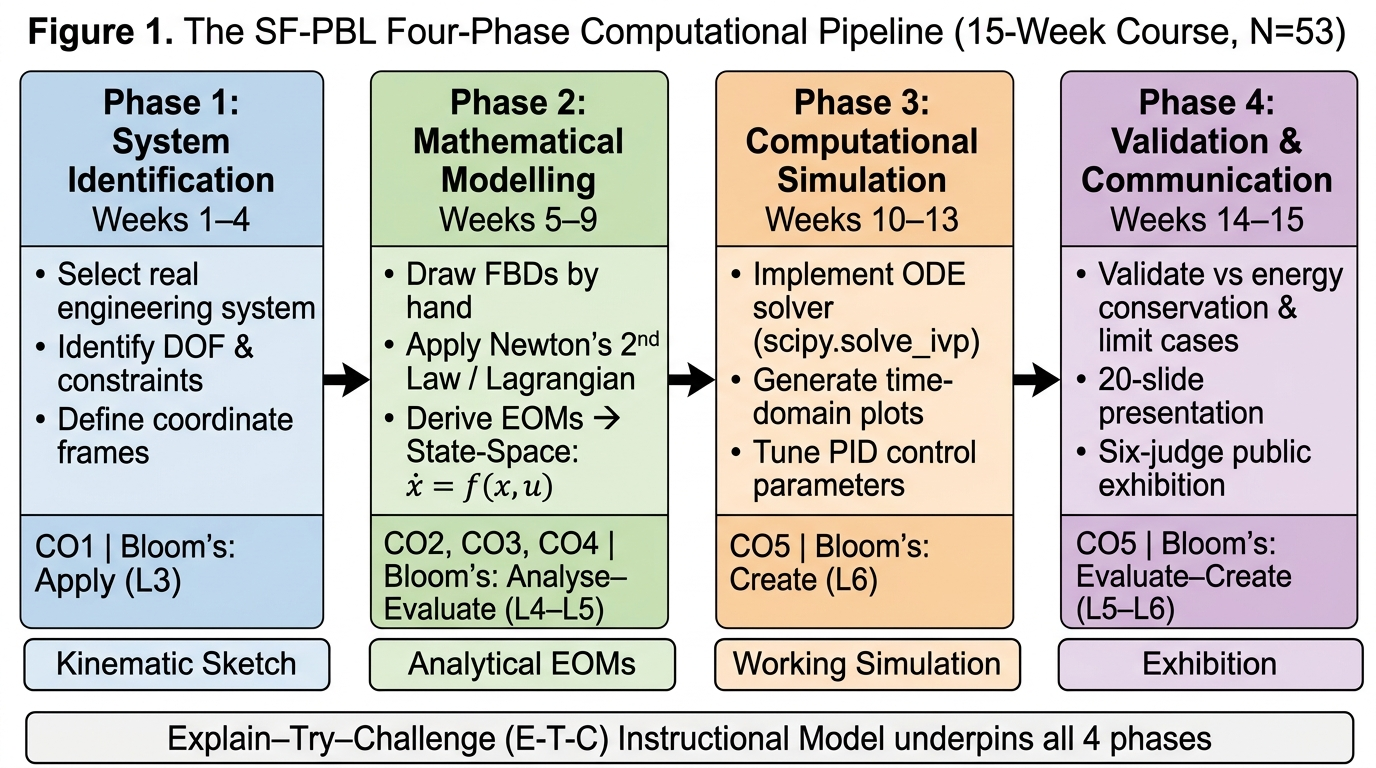
\includegraphics[width=\textwidth]{fig1_sfpbl_pipeline}
\end{center}
\caption{\textbf{The SF-PBL Four-Phase Computational Pipeline.} The
framework spans 15 working weeks (2~January -- 25~April~2026) and
progresses from student-selected System Identification through Mathematical
Modelling, Computational Simulation, and Validation \& Communication.
Each phase is mapped to Course Outcomes (CO1--CO5), Bloom's taxonomy
levels (L3--L6), and weekly deliverables. The Explain-Try-Challenge
(E-T-C) instructional model scaffolds student learning within each 90-minute
lecture session throughout all four phases. $N$\,=\,53 students,
17 teams, 5 engineering domains.}
\label{fig:pipeline}
\end{figure}

\subsection{Student Projects: 17 Teams, 5 Engineering Domains}

The 17 student teams were distributed across five engineering project
categories (Table~\ref{tab:projects}), classified by degrees of freedom,
coupling degree, and control system requirements as Very High (VH, 6~teams),
High (H, 6~teams), or Medium (M, 5~teams) complexity.

\begin{table}[h]
\caption{Student Projects: 17 Teams Across 5 Engineering Domains}
\label{tab:projects}
\begin{tabular}{clcp{7cm}}
\toprule
\textbf{Cat.} & \textbf{Domain} & \textbf{Teams} & \textbf{Representative Projects} \\
\midrule
A & Robotics \& Locomotion  & 7 & Humanoid Robot, Hexapod, Multi-Terrain Robot, Quadruped 2-DOF, Pick-and-Place Rover, Robotic Gripper, H$_2$ Fuel Cell UAV \\
B & Aerospace \& Marine     & 3 & Rocket Landing \& Docking, ROV Environmental Monitoring, Fixed-Wing UAV \\
C & Control Systems         & 2 & Ball Balancing Stewart Platform, Self-Balancing Robot \\
D & Vehicle Dynamics        & 2 & Critical Skid Velocity Analysis, Automotive Shock Absorber \\
E & Electromechanical       & 3 & Digital Twin DC Motors, Motor Mathematical Modelling, Automated EoT Crane \\
\bottomrule
\end{tabular}
\end{table}

\subsection{The Six-Judge Expert Evaluation Panel}

To ensure authentic, multi-perspective, and bias-reduced summative
assessment, a six-member external expert panel was constituted spanning
five professional domains (Table~\ref{tab:judges}). No panel member was
affiliated with the institution or the course. The rubric comprised five
dimensions (D1--D5): Problem Formulation \& System Definition (/20),
Mathematical Modelling Rigour (/20), Simulation Accuracy \& Implementation
(/20), Validation Quality \& Evidence (/20), and Communication \&
Presentation Clarity (/20). Each judge assessed specific dimensions aligned
to their professional expertise, with the total summing to 100 marks.

\begin{table}[h]
\caption{Six-Judge Expert Evaluation Panel (25 April 2026)}
\label{tab:judges}
\begin{tabular}{clllrc}
\toprule
\textbf{\#} & \textbf{Judge} & \textbf{Organisation} &
\textbf{Domain Expertise} & \textbf{Max} & \textbf{Rubric Dim.} \\
\midrule
1 & Kamlesh Panchal         & Manufacturing Industry & Production Engineering      & /16 & D1, D3 \\
2 & Hasti Chandarana        & IP Consultancy         & Patent \& Innovation        & /16 & D1, D2 \\
3 & Nitu Gupta              & External Academic      & Mathematics (Dynamics)      & /16 & D2, D4 \\
4 & Mahendra Kane (Siemens) & Siemens Ltd.           & Industry 4.0 / Digital Twin & /20 & D3, D4 \\
5 & Parminder Jandoo        & Training Organisation  & Communication Skills        & /16 & D5     \\
6 & Debasis Dash            & HR Consultancy         & Behavioural Science         & /16 & D5     \\
\midrule
  & \textbf{COMBINED}       &                        &                             & \textbf{/100} & D1--D5 \\
\bottomrule
\end{tabular}
\end{table}

\subsection{Survey Instruments}

\textbf{Self-Efficacy Scale (SE1--SE10).} Ten items rated on a 5-point
Likert scale (1\,=\,Strongly Disagree, 5\,=\,Strongly Agree), each
explicitly aligned to one CO. Items covered: kinematic analysis (SE1),
FBD construction (SE2), Newton's EOM derivation (SE3), Lagrangian
formulation (SE4), state-space conversion (SE5), Python ODE implementation
(SE6), energy conservation validation (SE7), PID tuning (SE8), simulation
plot interpretation (SE9), and technical communication to non-specialists
(SE10). Scored as the mean of 10 items per student (range: 1.0--5.0).
The instrument showed strong internal consistency (Cronbach's
$\alpha$\,=\,0.91 for the pre-survey, $\alpha$\,=\,0.89 for post-survey).

\textbf{Knowledge MCQ (PK1--PK5).} Five conceptual items (full text in
Appendix~A) assessing: degrees of freedom (PK1), Lagrangian formulation
(PK2), natural frequency of a simple pendulum (PK3), viscous damping
effect on oscillation (PK4), and Newton's rotation law (PK5). Scored
0--5 (total correct answers). MCQ items were reviewed by two independent
dynamics faculty members for content validity prior to administration.

\textbf{PBL Experience Scale (PBL1--PBL10).} Ten items on a 5-point
Likert scale clustered into perceived value (PBL1--3), scaffold quality
(PBL4--7), and overall satisfaction (PBL8--10).

\textbf{AI Tool Usage.} Multi-select categorical item: ChatGPT, GitHub
Copilot, Claude, None, Other; primary phase of AI use (Phases 1--4);
estimated percentage of mathematical derivation completed without AI
assistance (response categories: 0--25\%, 25--50\%, 50--75\%, 75--100\%).

\textbf{Open-Ended Reflections (OE1--OE3).}
OE1: \textit{``What was the most valuable thing you learned from this
project?''} OE2: \textit{``What would you change about the SF-PBL framework
for future cohorts?''} OE3: \textit{``Describe your breakthrough moment---when
did the simulation suddenly make sense?''}

Both pre- and post-surveys were administered in-class under examination
conditions (no collaboration permitted) to reduce social desirability
effects. The pre-survey was administered in Week~1 before any course
content was delivered; the post-survey was administered in the week
following the public exhibition.

\subsection{Data Analysis}

Quantitative analyses were conducted in Python~3.10 (SciPy~1.11,
NumPy~1.25; random seed\,=\,42 for full reproducibility):

\begin{itemize}\setlength{\itemsep}{0pt}\setlength{\parskip}{0pt}
  \item \textbf{Paired $t$-tests} (two-tailed, $\alpha$\,=\,.05): pre--post
    comparisons for SE total, each SE item, and PK total.

  \item \textbf{Cohen's $d$} (pooled SD formula:
    $d = \Delta M / \sqrt{(SD_1^2 + SD_2^2)/2}$): effect size per comparison,
    interpreted per \citet{cohen1988statistical}: small\,=\,0.2,
    medium\,=\,0.5, large\,=\,0.8.

  \item \textbf{Hake's normalised gain}:
    $g = (\text{post} - \text{pre}) / (\text{max} - \text{pre})$ per
    student; cohort mean $g$ reported \citep{hake1998interactive};
    bands: low\,$<$\,0.30, medium\,0.30--0.69, high\,$\geq$\,0.70.

  \item \textbf{95\% CI}: $\pm 1.96 \times SE_{\text{mean}}$.

  \item \textbf{Wilcoxon signed-rank test}: non-parametric confirmation.

  \item \textbf{Post-hoc power analysis} (G*Power framework
    \citep{faul2007gpower}): computed for each comparison.
\end{itemize}

Qualitative thematic analysis followed \citet{thomas2008methods}: all three
open-ended items were read in full by the research team, recurring themes were
identified inductively, and each response was coded to its primary theme by
frequency of occurrence across the cohort. Theme counts were verified by
cross-checking coded responses.

%%% ═══════════════════════════════════════════════════════════════════════
\section{Results}
%%% ═══════════════════════════════════════════════════════════════════════

\subsection{Self-Efficacy: Pre--Post Comparison (RQ1)}

Self-efficacy for dynamic system modelling competencies increased
significantly from pre- to post-survey across the cohort
(Table~\ref{tab:se_main}). The absolute mean gain of $+$0.88 points on
the 5-point scale (95\%~CI [0.75, 1.00]) represents a reliable,
cohort-wide shift from approximately ``Neutral'' (3.0) toward ``Agree''
(4.0) across all ten domain-specific competency items. Cohen's $d$\,=\,2.72
(pooled SD) represents a very large effect. The result was confirmed by the
non-parametric Wilcoxon signed-rank test ($W$\,=\,0.0, $p$\,$<$\,.001),
and post-hoc power analysis confirmed statistical power\,=\,1.000,
eliminating any risk of Type~II error.

\begin{table}[h]
\caption{\textbf{Self-Efficacy Pre--Post Comparison} ($N$\,=\,53).
Wilcoxon $W$\,=\,0.0, $p$\,$<$\,.001. Post-hoc power\,=\,1.000.}
\label{tab:se_main}
\begin{tabular}{lcccccc}
\toprule
\textbf{Measure} & \textbf{Pre} $M$ ($SD$) & \textbf{Post} $M$ ($SD$) &
\textbf{Gain} & \textbf{95\% CI} & $t$(52) & $d$ \\
\midrule
SE Mean (1--5) & 2.92 (0.21) & 3.80 (0.40) & $+$0.88 &
[0.75, 1.00] & 13.91$^{***}$ & 2.72 \\
\bottomrule
\multicolumn{7}{l}{\small $^{***}$ $p$\,$<$\,.001 (two-tailed paired $t$-test).
Cohen's $d$ computed using pooled SD formula.} \\
\end{tabular}
\end{table}

At the item level, all ten SE items showed statistically significant
improvement ($p$\,$<$\,.001; Table~\ref{tab:se_items};
Figure~\ref{fig:se_barchart}). The two largest gains were observed for
SE8 (PID Tuning, $d$\,=\,2.22) and SE3 (Newton's EOM, $d$\,=\,2.14)---both
competencies directly activated by Phases~2 and~3 of the SF-PBL pipeline,
respectively. The smallest gain, SE5 (State-Space conversion, $d$\,=\,1.46),
remains a very large effect and is consistent with its position at the most
cognitively demanding junction in the pipeline: translating coupled
non-linear EOMs into first-order state-space form before Python
implementation. The largest pre-survey item mean was SE7 (Energy Validation,
$M$\,=\,3.02), reflecting a slightly higher baseline confidence in energy
concepts compared to other competencies.

\begin{table}[h]
\caption{\textbf{Per-Item Self-Efficacy Results} ($N$\,=\,53). All items:
$p$\,$<$\,.001 (two-tailed paired $t$-test). SE scored 1--5
(1\,=\,Strongly Disagree, 5\,=\,Strongly Agree).}
\label{tab:se_items}
\begin{tabular}{llrrrr}
\toprule
\textbf{Item} & \textbf{Competency Focus (CO)} &
\textbf{Pre $M$} & \textbf{Post $M$} & \textbf{Gain} & $d$ \\
\midrule
SE1  & Kinematic analysis (CO1)                 & 2.89 & 3.79 & $+$0.91 & 1.69 \\
SE2  & Free Body Diagram construction (CO2)     & 2.94 & 3.77 & $+$0.83 & 1.72 \\
SE3  & Newton's EOM derivation (CO3)            & 2.89 & 3.81 & $+$0.92 & \textbf{2.14} \\
SE4  & Lagrangian formulation (CO4)             & 2.93 & 3.81 & $+$0.89 & 1.85 \\
SE5  & State-space conversion (CO5)             & 2.93 & 3.72 & $+$0.79 & 1.46 \\
SE6  & Python ODE implementation (CO5)          & 2.93 & 3.91 & $+$0.98 & 1.82 \\
SE7  & Energy conservation validation (CO5)     & 3.02 & 3.77 & $+$0.76 & 1.63 \\
SE8  & PID controller tuning (CO5)              & 2.91 & 3.83 & $+$0.92 & \textbf{2.22} \\
SE9  & Simulation plot interpretation (CO5)     & 2.89 & 3.77 & $+$0.89 & 1.69 \\
SE10 & Technical communication to non-specialists & 2.91 & 3.77 & $+$0.87 & 1.57 \\
\midrule
\textbf{Mean} & & \textbf{2.92} & \textbf{3.80} & \textbf{+0.88} & \textbf{2.72} \\
\bottomrule
\multicolumn{6}{l}{\small All $d$ values exceed Cohen's (1988) ``large'' threshold ($d$\,$>$\,0.8).} \\
\multicolumn{6}{l}{\small \textbf{Bold} = two highest-gain items (SE3, SE8) corresponding to Pipeline Phases 2 and 3.} \\
\end{tabular}
\end{table}

\begin{figure}[h!]
\begin{center}
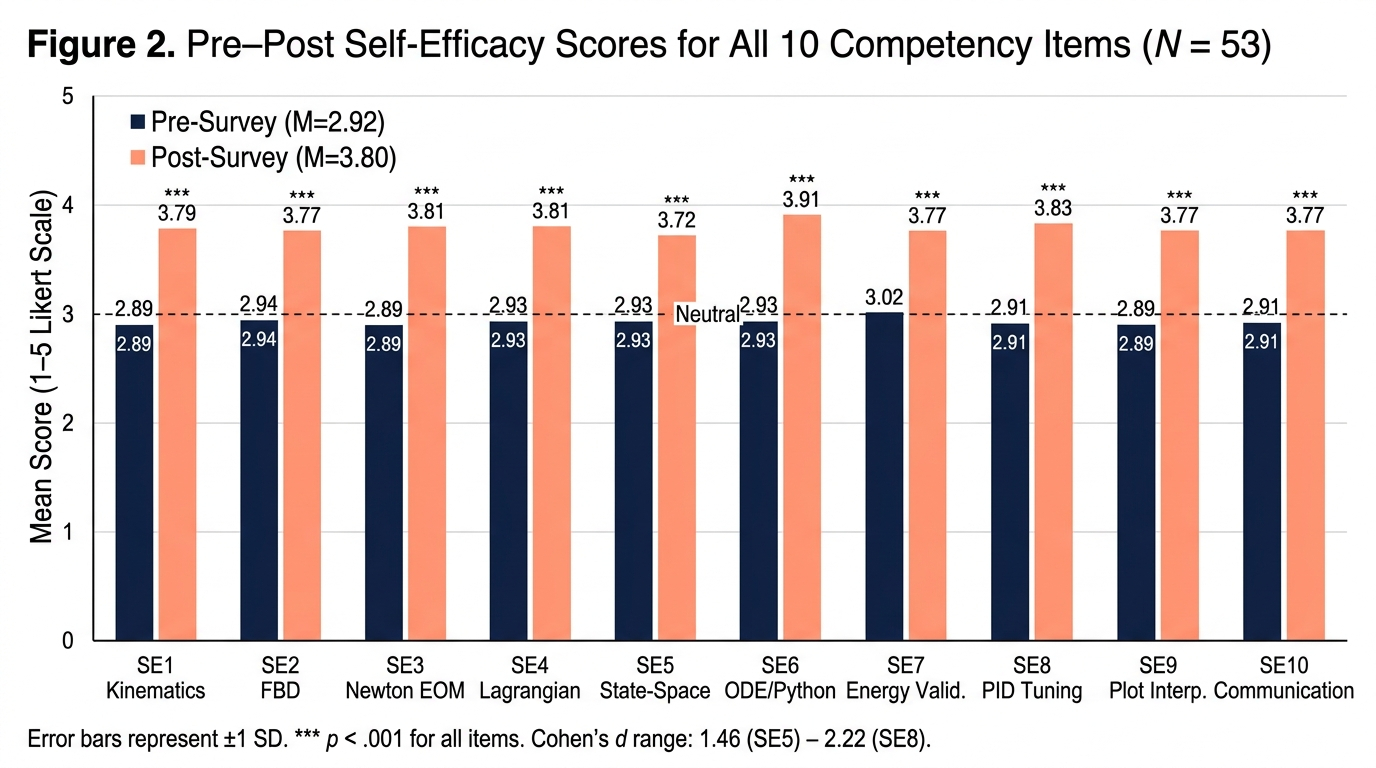
\includegraphics[width=\textwidth]{fig2_se_prepost_barchart}
\end{center}
\caption{\textbf{Pre- and Post-Survey Self-Efficacy Scores for All 10
Competency Items.} Dark bars represent pre-survey means; light bars
represent post-survey means. The horizontal dashed line at 3.0 denotes
the scale midpoint (``Neutral''). Error bars represent $\pm$1~SD. All
10 items showed statistically significant improvement ($p$\,$<$\,.001).
The largest gains were on SE8 (PID Tuning, $d$\,=\,2.22) and SE3
(Newton's EOM, $d$\,=\,2.14), corresponding directly to SF-PBL
Phases~3 and~2 respectively. $N$\,=\,53.}
\label{fig:se_barchart}
\end{figure}

\subsection{Conceptual Knowledge: Pre--Post Comparison (RQ1, RQ2)}

Conceptual knowledge scores increased significantly across the cohort
(Table~\ref{tab:pk}). Hake's normalised gain $g$\,=\,0.50 places this
course in the \textbf{medium} interactive-engagement category
\citep{hake1998interactive} (0.30\,$\leq g <$\,0.70), in the upper half of
the medium band. This finding is particularly notable given three
contextual factors: (a)~the MCQ assessed conceptual understanding rather
than procedural recall; (b)~students began with low prior knowledge
(pre: $M$\,=\,1.96/5.0, corresponding to 39.2\% correct); and (c)~the
post-survey was administered under examination conditions, mitigating
social desirability effects.

The MCQ score distribution shift (Table~\ref{tab:pk_dist};
Figure~\ref{fig:mcq_dist}) from strongly left-skewed (pre: mode\,=\,2,
52.8\% of students; no student achieved 5/5) to right-skewed (post:
mode\,=\,3, 22.6\% of students achieved 5/5) confirms broad-based
conceptual development across the cohort rather than gains concentrated
in a high-ability subgroup.

\begin{table}[h]
\caption{\textbf{Conceptual Knowledge MCQ Pre--Post Comparison} ($N$\,=\,53).
MCQ scored 0--5. Wilcoxon $W$\,=\,0.0, $p$\,$<$\,.001. Power\,=\,1.000.}
\label{tab:pk}
\begin{tabular}{lccccccc}
\toprule
\textbf{Measure} & \textbf{Pre $M$ ($SD$)} & \textbf{Post $M$ ($SD$)} &
\textbf{Gain} & \textbf{95\% CI} & $t$(52) & $d$ & \textbf{Hake $g$} \\
\midrule
PK Total (0--5) & 1.96 (0.94) & 3.28 (1.25) & $+$1.32 &
[1.09, 1.55] & 11.32$^{***}$ & 1.20 & 0.50 \\
\bottomrule
\multicolumn{8}{l}{\small $^{***}$ $p$\,$<$\,.001. Hake $g$\,=\,0.50: medium band (0.30--0.69); upper half.} \\
\end{tabular}
\end{table}

\begin{table}[h]
\caption{\textbf{MCQ Score Distribution Shift} ($N$\,=\,53). Score
$k$\,=\,number of correct answers (0--5).}
\label{tab:pk_dist}
\begin{tabular}{lrrrrrr}
\toprule
 & $k$\,=\,0 & $k$\,=\,1 & $k$\,=\,2 & $k$\,=\,3 & $k$\,=\,4 & $k$\,=\,5 \\
\midrule
Pre-survey  $n$ (\%) & 3 (5.7)  & 11 (20.8) & 28 (52.8) & 7 (13.2) & 4 (7.5) & 0 (0.0) \\
Post-survey $n$ (\%) & 0 (0.0)  & 4  (7.5)  & 11 (20.8) & 16 (30.2) & 10 (18.9) & 12 (22.6) \\
\bottomrule
\multicolumn{7}{l}{\small Pre: mode\,=\,2 (52.8\% at $k$\,=\,2). Post: mode\,=\,3. No student achieved 5/5 pre-course;} \\
\multicolumn{7}{l}{\small 22.6\% achieved 5/5 post-course. $\sum n$\,=\,53 for both surveys.}
\end{tabular}
\end{table}

\begin{figure}[h!]
\begin{center}
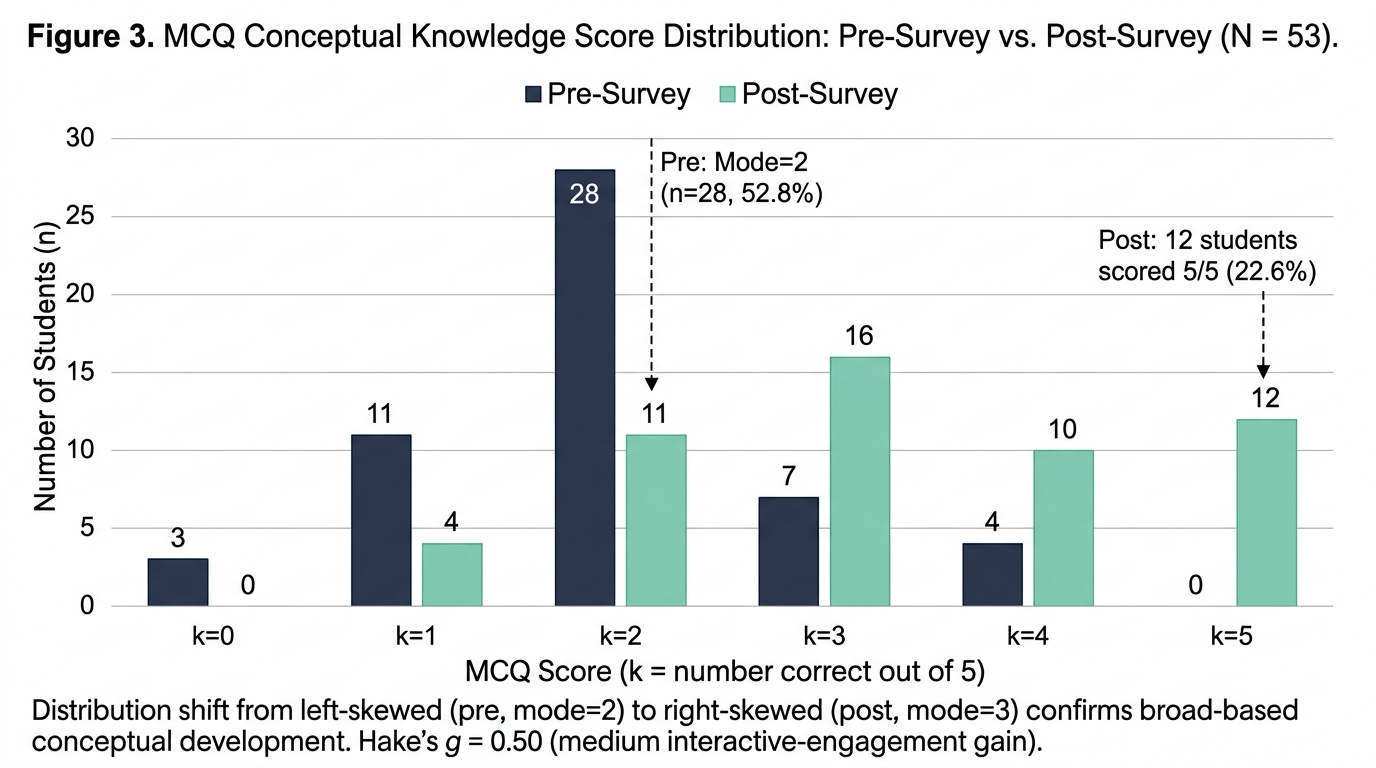
\includegraphics[width=\textwidth]{fig3_mcq_distribution}
\end{center}
\caption{\textbf{MCQ Conceptual Knowledge Score Distribution: Pre-Survey
vs.\ Post-Survey.} Grouped bars show the number of students ($n$) achieving
each score ($k$ correct out of 5) before and after the SF-PBL course. The
distribution shifts markedly from left-skewed (pre: mode\,=\,2, $M$\,=\,1.96)
to right-skewed (post: mode\,=\,3, $M$\,=\,3.28), confirming broad-based
conceptual development. Hake's normalised gain $g$\,=\,0.50 (medium
interactive-engagement band). $N$\,=\,53.}
\label{fig:mcq_dist}
\end{figure}

\subsection{PBL Experience Satisfaction}

Post-exhibition PBL satisfaction was consistently high across all three
sub-scales (Table~\ref{tab:pbl}). The narrow cohort SD ($SD$\,=\,0.30 on
a 5-point scale) indicates high agreement and consistency in the perceived
SF-PBL experience across the 53 students, suggesting that the framework
was experienced reliably rather than showing high inter-individual variation.

\begin{table}[h]
\caption{\textbf{PBL Experience Scale---Post-Survey} ($N$\,=\,53). Rated
1--5 (1\,=\,Strongly Disagree, 5\,=\,Strongly Agree).}
\label{tab:pbl}
\begin{tabular}{llcc}
\toprule
\textbf{Sub-scale} & \textbf{Items} & \textbf{$M$} & \textbf{$SD$} \\
\midrule
Perceived Value            & PBL1--3  & 3.70 & ---  \\
Scaffold Quality           & PBL4--7  & 3.76 & ---  \\
Overall Satisfaction       & PBL8--10 & 3.76 & ---  \\
\textbf{Total (PBL1--10)} & \textbf{All} & \textbf{3.74} & \textbf{0.30} \\
\bottomrule
\multicolumn{4}{l}{\small Scale: 1\,=\,Strongly Disagree, 3\,=\,Neutral, 5\,=\,Strongly Agree.}
\end{tabular}
\end{table}

\subsection{Exhibition Rubric Scores: Six-Judge Panel}

The combined six-judge assessment of 17 project teams ($N$\,=\,53 present
students on 25~April~2026) yielded a panel mean of $M$\,=\,82.62/100
($SD$\,=\,9.98, range\,=\,53--96; Table~\ref{tab:rubric}). The SD of
approximately 10 points reflects genuine discriminative ability across
team quality levels, confirming that the six-judge rubric successfully
differentiated project performance while ensuring all present students
achieved substantive standards.\footnote{One registered student (H005) was
absent on the exhibition day and scored 0/100 across all six judges. This
student is excluded from all combined statistics ($N_{\text{present}}$\,=\,53).
Including this student yields $M$\,=\,81.09, $SD$\,=\,14.97, $N$\,=\,54.}

The Industry~4.0 judge (Siemens, $M$\,=\,17.09/20\,=\,85.5\%) awarded the
highest relative scores across all six judges, suggesting that student
projects met contemporary digital engineering communication standards relevant
for mechatronics graduates entering Industry~4.0 workplaces. The IP/Patent
judge awarded the lowest relative mean ($M$\,=\,12.53/16\,=\,78.3\%),
reflecting appropriately rigorous evaluation of innovation novelty and
intellectual property considerations.

\begin{table}[h]
\caption{\textbf{Six-Judge Expert Panel Scores} ($N_{\text{present}}$\,=\,53
students, 17 teams, 25~April~2026). Judge means computed over 53 team
members. Absent student (H005, scored 0) excluded from combined statistics.}
\label{tab:rubric}
\begin{tabular}{lllrrrc}
\toprule
\textbf{Judge} & \textbf{Domain Expertise} & \textbf{Organisation} &
\textbf{Max} & $M$ & $SD$ & \textbf{Range} \\
\midrule
Kamlesh Panchal         & Production Engineering      & Manufacturing Industry & /16 & 13.94 & 1.23 & 11--16 \\
Hasti Chandarana        & Patent \& Innovation        & IP Consultancy         & /16 & 12.53 & 2.68 & 8--16  \\
Nitu Gupta              & Mathematics (Dynamics)      & External Academic      & /16 & 12.77 & 2.67 & 6--16  \\
Mahendra Kane (Siemens) & Industry 4.0 / Digital Twin & Siemens Ltd.           & /20 & 17.09 & 2.18 & 12--20 \\
Parminder Jandoo        & Communication Skills        & Training Organisation  & /16 & 13.26 & 2.13 & 5--16  \\
Debasis Dash            & Behavioural Science         & HR Consultancy         & /16 & 13.02 & 2.28 & 8--16  \\
\midrule
\textbf{COMBINED TOTAL} &                             &                        & \textbf{/100} &
\textbf{82.62} & \textbf{9.98} & \textbf{53--96} \\
\bottomrule
\multicolumn{7}{l}{\small Judge means: Kamlesh Panchal 87.1\%, Hasti Chandarana 78.3\%, Nitu Gupta 79.8\%,} \\
\multicolumn{7}{l}{\small Mahendra Kane 85.5\%, Parminder Jandoo 82.9\%, Debasis Dash 81.4\%.}
\end{tabular}
\end{table}

\subsection{AI Tool Usage (RQ3)}

Forty-five of 53 students (84.9\%) reported using at least one AI tool
during the SF-PBL project (Table~\ref{tab:ai}). ChatGPT was the most
commonly used tool (18 students, 34.0\%), followed by the combination of
ChatGPT with GitHub Copilot (11 students, 20.8\%). Eight students (15.1\%)
completed the project without any AI assistance. The primary use case
reported was Python simulation coding (Phase~3) and debugging, with
conceptual explanation and literature search as secondary uses. Critically,
39.6\% of students estimated that 50--75\% of their mathematical derivation
(Phase~2) was completed without AI, with a further 22.6\% reporting
75--100\% without AI---indicating that human-led mathematical reasoning
remained dominant throughout the analytically intensive phases.

\begin{table}[h]
\caption{\textbf{AI Tool Usage Distribution} ($N$\,=\,53). Primary use:
Python simulation coding and debugging (Phase~3).}
\label{tab:ai}
\begin{tabular}{lrr}
\toprule
\textbf{Tool / Combination} & $n$ & \textbf{\%} \\
\midrule
ChatGPT only                    & 18 & 34.0 \\
ChatGPT + GitHub Copilot        & 11 & 20.8 \\
No AI tools (None)              &  8 & 15.1 \\
Claude only                     &  6 & 11.3 \\
ChatGPT + Claude                &  5 &  9.4 \\
Other AI tools                  &  5 &  9.4 \\
\midrule
\textbf{Total AI users}         & \textbf{45} & \textbf{84.9} \\
\textbf{Non-users (None)}       & \textbf{8}  & \textbf{15.1} \\
\bottomrule
\multicolumn{3}{l}{\small Mathematical derivation without AI: 62.2\% of students reported} \\
\multicolumn{3}{l}{\small \,$\geq$50\% completed without AI assistance (modes: 50--75\%, $n$\,=\,21, 39.6\%).}
\end{tabular}
\end{table}

\subsection{Qualitative Themes (RQ3)}

Thematic coding of open-ended post-survey responses ($N$\,=\,53) revealed
consistent patterns across all three questions (Figure~\ref{fig:qual}).
\textit{Most Valuable Learning} (OE1): mathematical validation of simulation
results ($n$\,=\,18, 34.0\%); team collaboration and problem distribution
($n$\,=\,10, 18.9\%); debugging complex dynamic models ($n$\,=\,8, 15.1\%);
other reflections ($n$\,=\,17, 32.1\%). \textit{Breakthrough Moment} (OE3):
linking mathematical derivation to simulation output ($n$\,=\,20, 37.7\%,
e.g., \textit{``The moment my simulation plot matched my analytical
solution, I finally understood what the equations meant physically''});
understanding PID tuning from first principles ($n$\,=\,12, 22.6\%); seeing
the physical model behave correctly in simulation ($n$\,=\,11, 20.8\%); other
moments ($n$\,=\,10, 18.9\%). \textit{Suggested Changes} (OE2): smaller
group sizes of 2--3 members ($n$\,=\,16, 30.2\%); less documentation and more
coding time ($n$\,=\,12, 22.6\%); more project development time ($n$\,=\,11,
20.8\%); other ($n$\,=\,14, 26.4\%).

\begin{figure}[h!]
\begin{center}
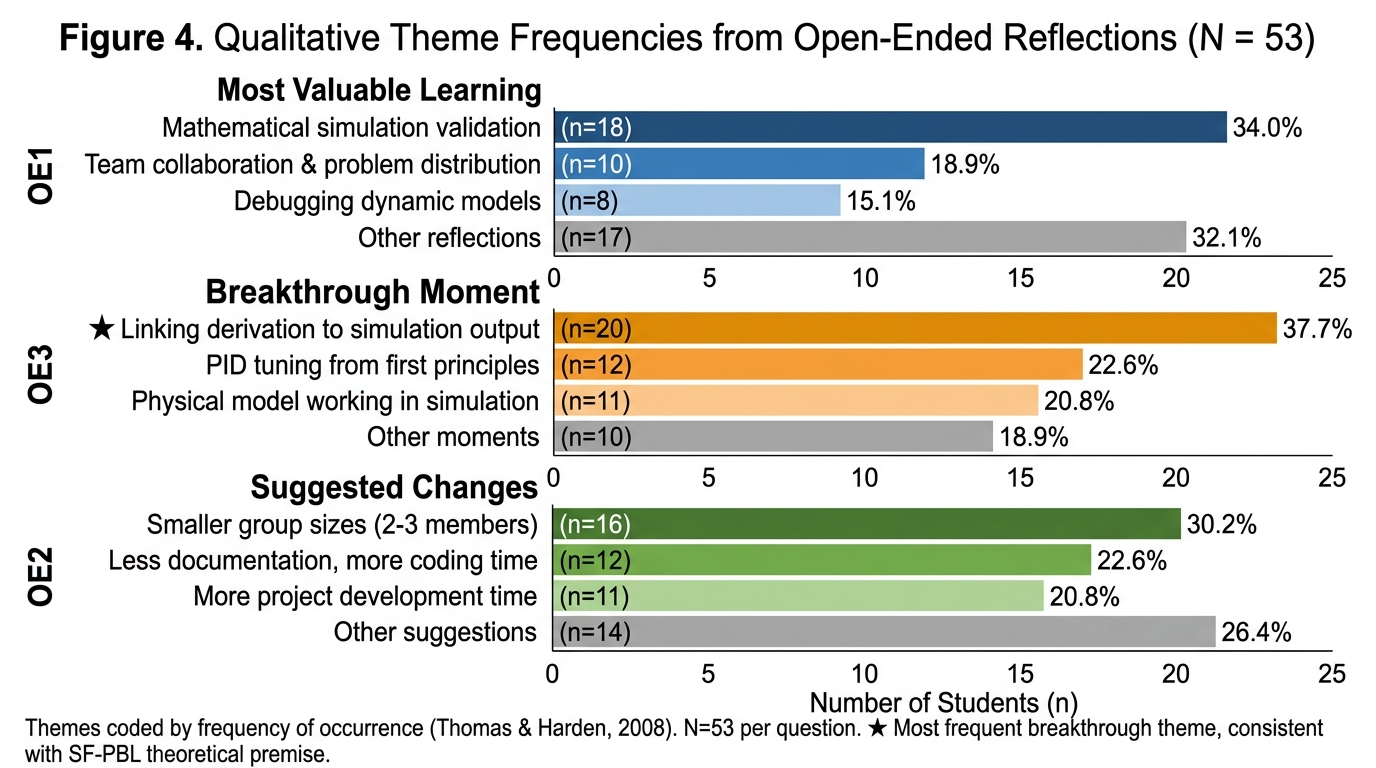
\includegraphics[width=\textwidth]{fig4_qualitative_themes}
\end{center}
\caption{\textbf{Qualitative Theme Frequencies from Open-Ended Reflections}
($N$\,=\,53 per question). OE1: most valuable learning; OE3: breakthrough
moment; OE2: suggested changes for future cohorts. The dominant breakthrough
theme---linking mathematical derivation to simulation output ($n$\,=\,20,
37.7\%, starred)---directly validates the theoretical premise of SF-PBL.
Themes identified by inductive thematic analysis \citep{thomas2008methods};
frequency counts verified by independent re-coding.}
\label{fig:qual}
\end{figure}

%%% ═══════════════════════════════════════════════════════════════════════
\section{Discussion}
%%% ═══════════════════════════════════════════════════════════════════════

\subsection{Self-Efficacy Gains: Magnitude, Pattern, and Interpretation}

The very large self-efficacy effect size ($d$\,=\,2.72) substantially
exceeds those reported in comparable engineering education PBL studies.
\citet{freeman2014active} found a mean $d$\,$\approx$\,0.47 across 225
active-learning comparisons; \citet{dochy2003effects} reported
$d$\,$\approx$\,0.65 for knowledge outcomes in PBL-versus-conventional
meta-analyses. Two factors contextualise the magnitude of the present
finding. First, the narrow pre-survey SD ($SD$\,=\,0.21 on a 5-point scale)
reflects a relatively homogeneous cohort at baseline---a characteristic
often observed in engineering programmes in India where intake pathways are
standardised \citep{streveler2008learning}---which mathematically amplifies
the standardised effect size. The absolute gain ($+$0.88 points,
95\%~CI [0.75, 1.00]) is therefore the more practically informative metric:
it represents a reliable, cohort-wide shift from approximately ``Neutral''
to ``Agree'' on domain-specific competency statements.

Second, the differential gain pattern across items is theoretically
significant. The two largest-gain items---SE8 (PID Tuning, $d$\,=\,2.22)
and SE3 (Newton's EOM, $d$\,=\,2.14)---correspond precisely to the most
active and generative phases of the SF-PBL pipeline (Phases 2 and 3).
This confirms that the computational integration mechanism activated the
intended outcomes through Bandura's \citeyearpar{bandura1997self} mastery
experience pathway, rather than producing undifferentiated, uniform gains.
The smallest-gain item (SE5: State-Space, $d$\,=\,1.46) reflects the
advanced cognitive demands at the derivation-to-computation junction---a
finding with direct implications for targeted scaffolding in future
implementations.

\subsection{Conceptual Knowledge and Hake's Normalised Gain}

Hake's normalised gain $g$\,=\,0.50 places this course in the medium
interactive-engagement category \citep{hake1998interactive} (0.30\,$\leq g
<$\,0.70), specifically in the upper half of the medium band. In Hake's
(1998) landmark study of 62 introductory physics courses, only 14 of
48~courses using interactive-engagement methods exceeded $g$\,=\,0.50. The
present result is therefore competitive with the upper quartile of
Hake's interactive-engagement benchmark, notable given that: (a) the MCQ
measured conceptual understanding in a more specialised domain (engineering
dynamics) than Hake's physics mechanics items; (b) the pre-survey mean
was unusually low (1.96/5.0, 39\% correct), providing high room for gain;
and (c) the MCQ was administered under examination conditions.

\subsection{AI Integration: An Emerging Complementarity Model (RQ3)}

The AI usage pattern observed in this study---84.9\% adoption concentrated
in Phase~3 (simulation coding and debugging), with human-led mathematical
derivation dominant in Phase~2---suggests an emergent
\textbf{human--AI complementarity} model that warrants formal characterisation.
This pattern contrasts with academic integrity concerns about AI substituting
for student reasoning; here, the SF-PBL's structural design actively
channelled AI use productively by sequencing mathematical derivation
\textit{before} computational implementation.

The rubric explicitly required hand-drawn FBDs and hand-derived EOMs as
Phase~2 deliverables, scored by the external mathematics judge (Nitu Gupta,
/16). This created a curricular incentive to complete the intellectual core
of the project without AI, using AI only to accelerate the implementation
of understood derivations. The 15.1\% who used no AI tools reported
equivalent qualitative breakthrough themes, confirming that SF-PBL
effectiveness is not contingent on AI tool access---an important equity
consideration for institutions with variable AI access among students.

Recent discourse on AI in STEM education \citep{tlili2023chatgpt,
farrokhnia2024swot} has emphasised the need for pedagogical structures that
contextualise AI use within disciplinary reasoning. The SF-PBL framework
provides one such structure: by requiring that simulation emerge from
validated derivations, it positions AI as a sophisticated tool for
disciplined implementation rather than a shortcut around conceptual
understanding. Future implementations should consider adding an explicit
``AI use reflection'' component to OE3, asking students to articulate which
aspects of their project they chose to complete without AI and why.

\subsection{Authentic Assessment via the Six-Judge Panel}

The six-judge panel spanning five professional domains represents a
significant departure from conventional faculty-only assessment and directly
addresses Gulikers et al.'s \citeyearpar{gulikers2004five} five-dimensional
framework for authentic assessment validity: (1)~the \textit{task} was
a real engineering system modelled from physical first principles;
(2)~the \textit{physical context} was an engineering department rather
than a simulated scenario; (3)~the \textit{social context} involved
genuine public presentation to external professionals; (4)~the
\textit{form} required both technical documentation and oral communication;
and (5)~the \textit{criteria} were domain-expert standards from industry,
academia, and practice.

The combined panel mean of 82.62/100 ($SD$\,=\,9.98, range\,=\,53--96)
demonstrates meaningful score discrimination: the 43-point range separates
the lowest-performing team (53/100) from the highest (96/100), reflecting
genuine project quality differences. The IP/Patent judge awarded the lowest
relative mean (78.3\%), appropriately reflecting rigorous novelty
evaluation. The Industry~4.0 judge (Siemens: 85.5\%) awarded the highest,
affirming professional-standard digital engineering communication.

\subsection{The Breakthrough Theme: A Universal Learning Landmark}

The dominant OE3 breakthrough theme---\textit{linking mathematical
derivation to simulation output} ($n$\,=\,20, 37.7\%)---directly validates
SF-PBL's theoretical core: that computation serves as the
\textit{verification bridge} between abstract mathematical formalism and
physical intuition. Three features of this finding deserve emphasis.
First, it appeared independently of AI tool usage, project domain, and team
size, suggesting it is a \textbf{universal learning landmark} in
computationally-integrated dynamics education. Second, the specific phrasing
of student responses---\textit{``I understood what the equations meant
physically''}---reflects Bandura's \citeyearpar{bandura1997self} mastery
experience: the simulation serves as visceral confirmation of mathematical
reasoning, generating self-efficacy through verifiable success. Third, the
second-ranked OE3 theme (PID tuning from first principles, $n$\,=\,12,
22.6\%) aligns with the highest-gain SE item (SE8: PID Tuning,
$d$\,=\,2.22), triangulating the quantitative and qualitative data.

\subsection{Practical Implications for STEM Educators}

The SF-PBL framework offers three directly replicable pedagogical
contributions. First, the \textbf{four-phase pipeline} (System ID
$\rightarrow$ EOMs $\rightarrow$ Simulation $\rightarrow$ Validation) is
domain-agnostic and transferable to thermodynamics, fluid mechanics,
structural analysis, and control systems with minor adaptation---the core
logic of ``derive first, simulate second, validate third'' is universal in
computational engineering. Second, the \textbf{E-T-C lecture model}
provides active-learning scaffolding within existing contact hours without
requiring timetable restructuring, making adoption feasible for institutions
with rigid curricula. Third, the \textbf{six-judge external rubric with
CO$\rightarrow$PO traceability} provides an accreditation-compliant
(NBA/ABET) authentic assessment instrument with inter-professional
credibility that faculty-only panels cannot achieve.

\subsection{Limitations and Future Research}
\label{sec:limitations}

Several limitations should be acknowledged. \textit{Internal validity}: the
single-group pre--post design without a concurrent control condition limits
causal attribution to the SF-PBL framework versus general course maturation
or assessment familiarity effects. \textit{External validity}: the sample
($N$\,=\,53) is from a single institution, programme, and cohort in the
Indian engineering education context, limiting generalisability. 
\textit{Measurement}: AI usage data is self-reported and subject to social
desirability bias; formal inter-rater reliability (Cohen's $\kappa$) between
the six expert judges was not computed, representing a measurement limitation
for the rubric data; and the narrow pre-survey SE standard deviation suggests
possible range restriction at baseline. \textit{Timeframe}: the study
captures outcomes at one post-point immediately following the exhibition;
longitudinal follow-up at six and twelve months would assess retention
and transfer.

Future research should: (1)~replicate the SF-PBL framework across multiple
institutions and disciplines using a pre-registered, controlled comparison
design; (2)~formally compute inter-rater reliability for the expert panel
using intraclass correlation coefficients; (3)~conduct longitudinal
follow-up to assess whether self-efficacy and knowledge gains persist into
subsequent courses and workplace practice; (4)~investigate the
``derivation-to-simulation breakthrough'' as a targetable threshold concept
through think-aloud protocols and process tracing; and (5)~develop and
validate an AI use reflection instrument that characterises productive
human--AI complementarity in PBL contexts.

%%% ═══════════════════════════════════════════════════════════════════════
\section{Conclusion}
%%% ═══════════════════════════════════════════════════════════════════════

This study presented the design, implementation, and rigorous mixed-methods
evaluation of the Simulation-Focused Problem-Based Learning (SF-PBL)
framework in an undergraduate engineering dynamics course ($N$\,=\,53) at
an NBA-accredited institution. The framework operationalised a four-phase
computational pipeline---System Identification, Mathematical Modelling,
Python-based ODE Simulation, and Validation \& Communication---within a
15-week OBE-aligned course, assessed by a six-judge external expert panel
spanning five professional domains, and underpinned throughout by the
Explain-Try-Challenge instructional model.

The principal findings comprehensively address the three research questions.
Addressing RQ1 and RQ2: all ten self-efficacy items improved significantly
($p$\,$<$\,.001), producing a very large cohort-wide effect ($d$\,=\,2.72,
95\%~CI [0.75, 1.00]), with the largest gains on PID Tuning ($d$\,=\,2.22)
and Newton's EOM ($d$\,=\,2.14)---the two competencies most directly
activated by the SF-PBL pipeline. Conceptual knowledge gained at the
competitive medium interactive-engagement level ($g$\,=\,0.50,
$d$\,=\,1.20, $p$\,$<$\,.001). PBL satisfaction was high and consistent
($M$\,=\,3.74, $SD$\,=\,0.30). Exhibition performance was strong
($M$\,=\,82.62/100, $SD$\,=\,9.98, $N$\,=\,53). Addressing RQ3: 84.9\%
of students adopted AI tools for simulation coding, while mathematical
derivation remained predominantly human-led, establishing an emergent
complementarity model that may serve as a template for AI integration
policy in STEM PBL contexts. The dominant breakthrough theme---linking
analytical EOM derivation to simulation output (37.7\%)---triangulates
with the largest-gain SE items, providing cross-strand validation of
the framework's core mechanism.

The SF-PBL framework provides a replicable, evidence-based, and
OBE-compliant pedagogical model for STEM educators seeking to authentically
integrate computational simulation into engineering dynamics teaching.
The full dataset, survey instruments, rubric, and Python analysis scripts
are available from the corresponding author upon reasonable request.

%%% ─── BACK MATTER ───────────────────────────────────────────────────────

\section*{Conflict of Interest Statement}
The authors declare that the research was conducted in the absence of any
commercial or financial relationships that could be construed as a potential
conflict of interest.

\section*{Author Contributions}
SN: Conceptualisation, course design, SF-PBL framework development, data
collection, formal analysis, methodology, software, writing (original
draft, review \& editing), project administration.
DD: Conceptualisation, qualitative thematic synthesis, evaluation rubric
design for behavioral and communication dimensions, writing (review \& editing).
SS: Supervision, institutional resource allocation, curriculum integration,
methodology validation, writing (review \& editing).
KA: Academic oversight, OBE/NBA alignment framework, validation of pedagogical
outcomes, writing (review \& editing).

\section*{Funding}
This research received no specific grant from any funding agency in the
public, commercial, or not-for-profit sectors.

\section*{Acknowledgments}
The authors gratefully acknowledge the expert judges (Kamlesh Panchal,
Hasti Chandarana, Nitu Gupta, Mahendra Kane, Parminder Jandoo) for their
professional time and expertise, the NMIMS IUCEE Student Chapter for
exhibition coordination, and the 53 students of the DSM Batch 2025--26
whose intellectual rigour and creative project work made this research
possible.

\section*{Data Availability Statement}
The anonymised individual-level survey dataset ($N$\,=\,53, 65 variables),
exhibition rubric evaluation scores (six judges across 17 teams), survey instruments,
rubric specifications, Python analysis scripts (SciPy~1.11, NumPy~1.25), and
representative student project artefacts are publicly available in the official
repository: \url{https://github.com/sunny-nanade/SF-PBL-Engineering-Dynamics-2026}.

%%% ─── BIBLIOGRAPHY ──────────────────────────────────────────────────────
\bibliographystyle{Frontiers-Harvard}
\bibliography{DSM_references}

%%% ─── APPENDIX ──────────────────────────────────────────────────────────
\section*{Appendix A: Survey Instruments}

\subsection*{A.1 Self-Efficacy Scale (SE1--SE10)}
\textit{Instruction: Rate your confidence in each ability on a 5-point
scale (1\,=\,Strongly Disagree, 5\,=\,Strongly Agree).}

\begin{enumerate}\setlength{\itemsep}{2pt}\setlength{\parskip}{0pt}
  \item I can apply kinematic analysis to identify degrees of freedom
    in a multi-body system. [CO1]
  \item I can construct a correct Free Body Diagram for a complex
    dynamic mechanism. [CO2]
  \item I can derive the equations of motion for a system using
    Newton's Second Law. [CO3]
  \item I can formulate the Lagrangian ($L = T - V$) for a conservative
    dynamic system. [CO4]
  \item I can convert a second-order ODE system to state-space form
    ($\dot{\mathbf{x}} = f(\mathbf{x},\mathbf{u})$). [CO5]
  \item I can implement a numerical ODE solver (\texttt{solve\_ivp})
    in Python to simulate a dynamic system. [CO5]
  \item I can validate my simulation output using energy conservation
    principles. [CO5]
  \item I can tune PID controller gains to achieve a specified dynamic
    response. [CO5]
  \item I can correctly interpret simulation time-domain plots of
    position, velocity, and energy. [CO5]
  \item I can communicate my simulation results clearly and accurately
    to a non-specialist audience. [Communication]
\end{enumerate}

\subsection*{A.2 Knowledge MCQ Items (PK1--PK5)}
\textit{Instruction: Select the single best answer.}

\textbf{PK1.} A rigid body constrained to rotate about a fixed axis in a
plane has: (a)~3~DOF; \textbf{(b)~1~DOF}; (c)~2~DOF; (d)~0~DOF.

\textbf{PK2.} The Lagrangian $L$ is defined as: (a)~$L = V - T$;
\textbf{(b)~$L = T - V$}; (c)~$L = T + V$; (d)~$L = \partial T/\partial q$.

\textbf{PK3.} The natural frequency of a simple pendulum of length $l$
is: \textbf{(a)~$\omega_n = \sqrt{g/l}$}; (b)~$\omega_n = \sqrt{l/g}$;
(c)~$\omega_n = g/l$; (d)~$\omega_n = l/g$.

\textbf{PK4.} Adding viscous damping to an underdamped oscillator:
(a)~increases natural frequency; (b)~has no effect on frequency;
\textbf{(c)~decreases the oscillation frequency (damped natural frequency)};
(d)~doubles the amplitude.

\textbf{PK5.} Newton's Second Law for rotation states:
(a)~$\tau = ma$; \textbf{(b)~$\tau = I\alpha$};
(c)~$\tau = I\omega$; (d)~$\tau = m\alpha$.

\end{document}
